Il presente capitolo ha lo scopo di introdurre il background metodologico su cui si basa il progetto di tesi sviluppato. Nella prima sezione verranno illustrati dei concetti fondamentali che ci aiuteranno a capire nel modo migliore quello che è stato fatto, chiaramente quello illustrato è una sintesi semplificata, la cui descrizione esaustiva e formale (decisamente più complessa) non è rilevante ai fine della comprensione di questa tesi. Nella seconda sezione rappresentiamo il movimento e l'orientamento degli oggetti 3D. Nella terza sezione verrà illustrato come viene controllata una mesh e il modello adottato. Nella quarta sezione come viene trasferito un movimento da un modello ad un altro con diverse struttura e morfologia.

\section{Mesh 3D e rappresentazioni geometriche}
Una mesh è un struttura di dati geometrici che segue la rappresentazioni di suddivisioni superficiali da un insieme di poligoni. Meshes sono particolarmente usate in computer graphics, per rappresentare superfici, o nella modellazione, per discretizzare una superficie continua o implicita ~\cite{mesh03}. Questa mesh può anche essere considerata come la combinazione geometrica e topologica, dove la geometrica fornisce le posizioni di tutte i vertici, e la topologia fornisce le informazioni tra differenti vertice adiacenti.

\begin{figure}
\begin{center}
     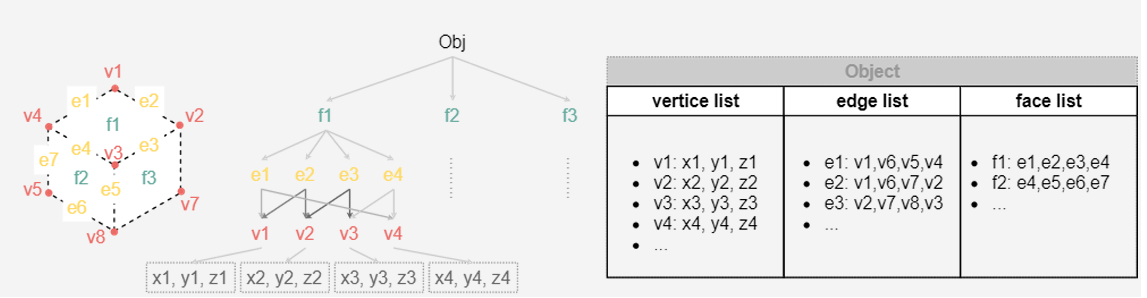
\includegraphics[width=12cm]{figure/mesh.png}
     \caption{La schematizzazione della rappresentazione di una mesh}
     \label{fig:mesh}
\end{center}
\end{figure}

\subsection{Vertici, lati, facce e struttura topologica}
Una mesh superficiale poligonale ha tre differenti elementi combinati: vertici, bordi e lati. La figura mostra gli elementi~\ref{fig:mesh}. Matematicamente ~\cite{mathmesh}, una mesh superficiale poligonale \(\mathcal{M}\) che contiene \(\mathcal{V}\) vertici e \(\mathcal{F}\) faccie è formato da:

\begin{align*}
\mathcal{M} = \{ (V, F) \mid 
V = \{ v_i \}_{i=1,2,\dots,V}, \;
F = \{ f_i \}_{i=1,2,\dots,F}, \;
f_i \in V^d
\}
\end{align*}

dove \(\mathcal{V}\) è l'insieme dei vertici , \(\mathcal{F}\) è l'insieme delle facce e d denota il numero di vertici di ogni faccia. Allo stesso modo, un volume di una mesh \(\mathcal{M}\) è formato da:

\begin{align*}
    \mathcal{M} = \{ (V,F,T) \mid
    T = \{ t_i \}_{i=1,2,\dots,t_i}, t_i \in F^k \}
\end{align*}

dove k rappresenta il numero di facce per ogni voxel t_i.

\subsection{Coordinate locali e globali, trasformazioni con matrici 4x4}
Tutti gli oggetti visualizzati in grafica 3D, si basano sulle posizioni dei loro vertici all'interno dello spazio tridimensionale. Queste coordinate però sono soggette a numerosi cambiamenti durante le animazioni.
Come visto, le coordinate rappresentano le posizioni dei vertici di una figura nello spazio 3D. Per visualizzare una scena, un programma di grafica deve conoscere le coordinate di tutti i vertici degli oggetti che devono essere visualizzati. Se l'oggetto viene spostato o ruotato, queste coordinate cambiano di conseguenza anche se la forma dell'oggetto rimane sempre la stessa.

Probabilmente la rappresentazione matriciali è più ottimale in termini di flessibilità, in quanto ti permette di rappresentare anche traslazione, scalature e altre trasformazioni. È, infatti, la rappresentazione che Blender utilizza internamente  proprio perché offre la maggior flessibilità. Siccome permette di rappresentare qualsiasi tipo di trasformazione, questa struttura viene solitamente chiamata \textit{Matrice di Trasformazione}. Nel caso caso di uno spazio a 3 dimensioni, essa a dimensione 4x4.~\cite{tec:2018}

Questa sua caratteristica la rende indispensable per rappresentare articolazoni formate da più ossa, che verrano illustrate di seguito ~\ref{fig:coord}, poichè rende possibile convertire le coordinate locali di un osso figlio a quelle locali del suo padre, fino ad arrivare alle coordinate globali.
%Per risolvere questo problema esistono due tipi di coordinate: Locali e Globali.
%Tutti gli oggetti sono descritti da un loro sistema di coordinate (coordinate locali) , quando vengono visualizzatti sulla scena, le loro coordinate vengono "trasformate" da locali a globali. Questa trasformazione, si può con un calcolo matematico concettualmente semplice (prodotto matrice - vettore).

\begin{figure}[H]
\begin{center}
     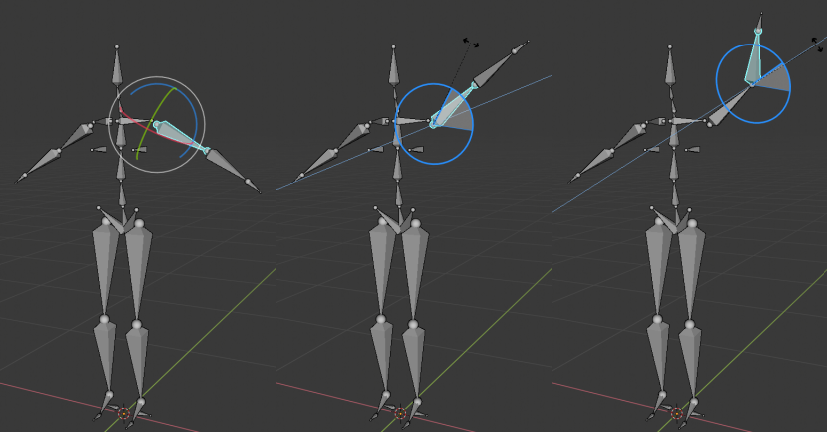
\includegraphics[width=12cm]{figure/coordi.png}
     \caption{La figura rappresenta la stessa armatura, formata da
diverse ossa, in tre posizioni differenti}
     \label{fig:coord}
\end{center}
\end{figure}



\subsection{Differenze tra mesh statica e mesh animata}
Una mesh statica è una struttura i cui vertici rimangono fissi nel tempo: rappresenta un oggetto immbile o privo di deformazioni, come un modello architettonico o un oggetto di scena.
Al contrario, una mesh animata varia la posizione dei suoi vertici nel tempo, secondo una serie di trasformazioni che possono derivare da:
\begin{enumerate}
    \item Animazione di oggetto (movimento rigido della mesh nel mondo)
    \item Rigging e skinning, dove i vertici sono influenzati da uno scheletro intero (armatura) e da pesi di deformazioni
    \item Simulazioni fisiche (tessuti, fluidi, soft body), in cui le posizioni vengono aggiornate dinamicamente.
\end{enumerate}
In pratica, una mesh animata non è solo una rappresentazione geometrica, ma un sistema dinamico che reagisce a vincoli, ossa  e forze esterne. La gestione efficiente di questa variazione temporale è ciò che rende possibile il movimento realistico nei personaggi e negli oggetti deformabili.

\section{Trasformazioni geometriche}
Nel contesto dell'animazione 3D, ogni elemento visivo - sia esso un personaggio o un oggetto - prende vita attraverso una combinazione di trasformazioni geometriche fondamentali: traslazione, rotazione e scalatura. Tali operazioni sono essenziali per finire le posizione, l'orientamento e la dimensione della mesh nello spazio tridimensionale, e vengono efficacemente rappresentate grazie all'uso di matrici 4x4 in coordinate omogenee. Queste matrici permettono la composizione sequenziale di più trasformazioni, garantendo un controllo elegante e coerente della deformazione e del movimento dei modelli.
Parallelamente, l'uso di quaternioni offre un'alternativa potente e matematicamente robusta per la reppresentazione delle rotazioni 3D: evitando problemi come il gimbal-lock, consentendo interpolazioni fluide e una gestione stabile dell'orientamento negli scheletri animati, i quaternioni si affermano come strumento preferito nei motori grafici e nei sistemi di animazione professionali.

Dal punto di vista matematico, tali trasformazioni vengono rappresentate mediante matrici 4x4, che consentono di gestire in modo unificato le operazioni dello spazio omogeneo. La composizione di più trasformazioni viene ottenuta attraverso la moltiplicazione delle rispettive matrici, seguendo in ordine preciso che influisce direttamente sul risultato finale.

Nell'ambito dell'animazione, queste trasformazioni vengono applicate in modo dinamico per determinare la posizione e la deformazione degli oggetti nel tempo. Ad esempio, durante un movimento di un personaggio, le trasformazioni delle singole ossa del rig vengono propagate alla mesh collegata, consentendo la corretta animazione della superficie. In questo senso, le trasformazioni rappresentano il collegamento diretto tra la rappresentazione matematica e il comportamento visivo del modello tridimensionale.

%\begin{figure}[h]
%\begin{center}
 %    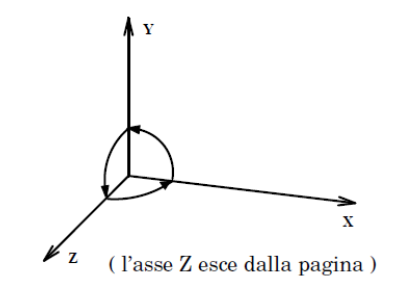
\includegraphics[width=8cm]{figure/asse.png}
  %   \caption{}
%\end{center}
%\end{figure}

\subsection{Traslazione, rotazione e scala 3D: rappresentazione matriciale e composizione}
Nel contesto della grafica e dell'animazione tridimensionale, ogni oggetto nello spazio virtuale è definito da un serie di coordinate che ne descrivono la posizione, l'orientamento e le dimensioni. 
Per modificare queste proprietà si utilizzano le trasformazioni geometriche, operazioni matematiche che permettono di spostare (traslazione), ruotare (rotazione) o ridimensionare (scala) un modello 3D mantenendo la coerenza spaziale della scena.

Tutte queste trasformazioni possono essere rappresentate mediante matrici 4x4, che consentono di combinare un'unica struttura i cambiamenti di posizione, orientamento e scala ~\cite{tras}. Questa rappresentazione matriciale è alla base della pipeline grafica moderna (in Blender, Unity e altri ambienti), poiché permette di applicare in modo efficiente e compatto più trasformazioni in sequenza attraverso la composizione matriciale.
Di seguito vengono descritte le tre principali trasformazioni elementari che definiscono il comportamento spaziale di una mesh o di un rig:

\begin{itemize}
    \item \textbf{Traslazione 3D}

La traslazione indica lo spostamento dell'oggetto lungo gli assi cartesiani
\begin{align*}
    T(d_x,d_y,d_z)
=
\begin{bmatrix}
    1 & 0 & 0 & d_x \\
    0 & 1 & 0 & d_y \\
    0 & 0 & 1 & d_z \\
    0 & 0 & 0 & 1 \\
\end{bmatrix}
\end{align*}

Infatti:\begin{align*}
    T (d_x,d_y,d_z)  \cdot \begin{bmatrix}x & y & z & 1\end{bmatrix}^T
    =
    \begin{bmatrix}
        x+d_x & y+d_y & z+d_z & 1 
    \end{bmatrix}^T
\end{align*}

\begin{figure}[h]
\begin{center}
     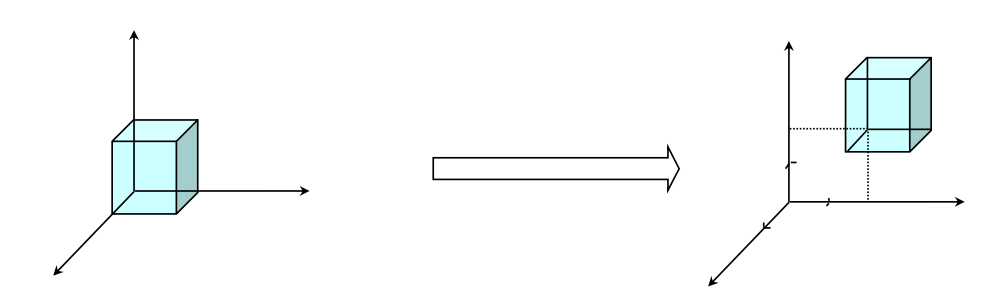
\includegraphics[width=12cm]{figure/trasla.png}
     \caption{Traslazione di un oggetto 3D}
\end{center}
\end{figure}

    \item \textbf{Rotazione 3D}
    
La rotazione definisce l'orientamento nello spazio, in questo caso è necessario definire tre rotazioni base, una attorno a ciuscuno dei tre assi x, y e z.

\begin{figure}[h]
\centering
\begin{minipage}{0.45\linewidth}
\centering
\begin{align*}
R_z(\theta) =
\begin{bmatrix}
\cos\theta & -\sin\theta & 0 & 0 \\
\sin\theta &  \cos\theta & 0 & 0 \\
0          &  0          & 1 & 0 \\
0          &  0          & 0 & 1
\end{bmatrix}
\end{align*}
\end{minipage}
\hfill
\begin{minipage}{0.45\linewidth}
\centering
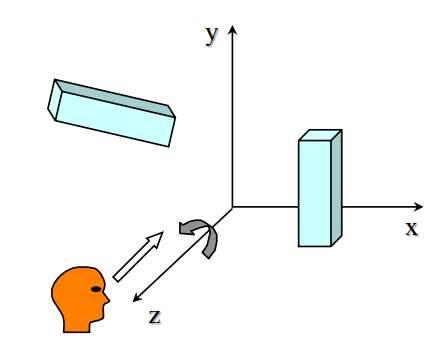
\includegraphics[width=\linewidth]{figure/rotazioneZ.png}
\end{minipage}
\caption{Matrice di rotazione $R_z(\theta)$ e visualizzazione 3D.}
\end{figure}

\begin{figure}[h]
\centering
\begin{minipage}{0.45\linewidth}
\centering
\begin{align*}
R_z(\theta) =
\begin{bmatrix}
1          & 0           & 0           & 0 \\
0          &  \cos\theta & -\sin\theta & 0 \\
0          &  \sin\theta & \cos\theta  & 0 \\
0          &  0          & 0           & 1
\end{bmatrix}
\end{align*}
\end{minipage}
\hfill
\begin{minipage}{0.45\linewidth}
\centering
\includegraphics[width=\linewidth]{figure/rotazioneX.png}
\end{minipage}
\caption{Matrice di rotazione $R_x(\theta)$ e visualizzazione 3D.}
\end{figure}



\begin{figure}[H]
\centering
\begin{minipage}{0.45\linewidth}
\centering
\begin{align*}
R_z(\theta) =
\begin{bmatrix}
\cos\theta & 0 & \sin\theta & 0 \\
0 &  1 & 0 & 0 \\
-\sin\theta          &  0          & \cos\theta & 0 \\
0          &  0          & 0 & 1
\end{bmatrix}
\end{align*}
\end{minipage}
\hfill
\begin{minipage}{0.45\linewidth}
\centering
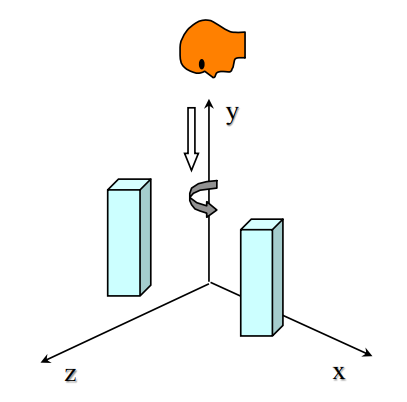
\includegraphics[width=\linewidth]{figure/rotazioneY.png}
\end{minipage}
\caption{Matrice di rotazione $R_y(\theta)$ e visualizzazione 3D.}
\end{figure}
   
\FloatBarrier  % assicura che la figura sia stampata

% item Scala 3D
\item \textbf{Scala 3D} \\[0.3em]
La scala determina l’ingrandimento o la riduzione lungo le diverse direzioni.

\[
S(s_x,s_y,s_z) =
\begin{bmatrix}
 s_x & 0 & 0 & 0 \\
 0 & s_y & 0 & 0 \\
 0 & 0 & s_z & 0 \\
 0 & 0 & 0 & 1
\end{bmatrix}
\]

Infatti:\begin{align*}
    S (s_x,s_y,s_z)  \cdot \begin{bmatrix}x & y & z & 1\end{bmatrix}^T
    =
    \begin{bmatrix}
        x \cdot s_x & y \cdot d_y & z \cdot s_z & 1 
    \end{bmatrix}^T
\end{align*}

\begin{figure}[h]
\begin{center}
     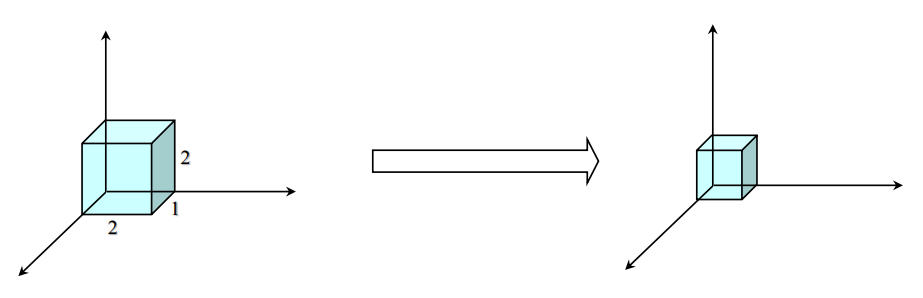
\includegraphics[width=12cm]{figure/scala.png}
     \caption{Scala di un oggetto 3D}
\end{center}
\end{figure}
    
\end{itemize}

\subsection{Rotazione con quaternioni: motivazione e vantaggi rispetto agli Euler angles (no gimbal lock)}
Nel contesto della grafica tridimensionale, le trasformazioni geometriche costituiscono la base matematica attraverso cui è possibile descrivere la posizione e l'orientamento di un oggetto nello spazio. Storicamente, tali trasformazioni sono state rappresentate mediante matrici di trasformazione, che agiscono come uno stato di riferimento o "base": moltiplicando un vettore o una matrice per la matrice di trasformazione corrispondente, è possibile ottenere la nuova posizione o orientazione dell'oggetto nello spazio tridimensionale.
Per la rappresentazione delle rotazioni, un approccio tradizionale è quello basato sugli angoli di Eulero, i quali definiscono l'orientamento di un corpo attraverso una sequenza ordinata di rotazioni elementari attorno agli assi principali del sistema di riferimento (X, Y, Z). Sebbene intuitivi e storicamente molto diffusi, gli angoli di Eulero presentano alcune limitazioni, tra cui in particolare la possibilità di incontrare configurazioni critiche che riducano la stabilità della rotazione.

Per superare tali problematiche, si è progressivamente affermato l'impiego dei \textbf{quaternioni}, una formulazione matematica più robusta ed efficiente per la gestione delle rotazioni tridimensionali. I quaternioni consentono di rappresentare in modo compatto un orientamento nello spazio e di calcolare rotazioni continue e interpolazioni fluide tra pose differenti, evitando le ambiguità e le discontinuità tipiche degli angoli di Eulero. La loro struttura, derivata dai numeri complessi, permette inoltre una maggiore stabilità numerica e una gestione più coerente delle rotazioni cumulative, rendendoli uno strumento esenziale nelle moderne pipeline di animazione e rigging.

\begin{itemize}
    \item \textbf {Angoli di Eulero}
    
    Gli angoli di Eulero rappresentano uno dei metodi più tradizionali per descrivere l'orientamento di un oggetto nello spazio tridimensionale. Essi contengono di esprimere una rotazione come una sequenza ordinata di tre rotazioni elementari attorno agli assi di un sistema di riferimento fisso, generalmente identificati come roll (x), pitch (y) e yaw (z).
    
    Questa rappresentazione è intuitiva, poiché ogni angolo corrisponde a una rotazione attorno ad un asse specifico, permettendo di comprendere facilmente il movimento nello spazio tridimensionale. Gli angoli di Eulero sono stati ampiamente utilizzati in diversi ambiti, tra cui la grafica computazionale, la robotica e l'ingegneria aerospaziale, grazie alla loro semplicità e compatibilità con numerosi software e framework.

    Tuttavia, tale rappresentazione soffre di limitazioni strutturali. In particolare, può verificarsi il fenomeno noto come gimbal lock, una condizione in cui due assi di rotazione diventano allineati, riducendo effettivamente i gradi di libertà del sistema. Questa degenerazione comporta instabilità numerica e ambiguità nell'orientamento, sopratutto quando si interagisce con pose molto articolate. Inoltre, l'ordine delle rotazioni (ad esempio, XYZ rispetto a ZYX) influenza direttamente il risultato finale, introducendo ulteriore ambiguità. ~\cite{quater}.

    Per queste ragioni, nonostante la loro accessibilità concettuale, gli angoli di Eulero sono oggi spesso sostituiti dai quaternioni, i quali garantiscono una rappresentazione continua, priva di singularità e dunque più adatta ai contesti di animazione e rigging avanzato.

    \item \textbf{Rotazione con Quaternioni}
    
    Nello spazio tridimensionale una rotazione può essere descritta specificando un asse e un angolo di rotazione. Seguendo la convenzione comunemente adottata, una rotazione con angolo positivo viene eseguita in senso antiorario rispetto alla direzione dell'asse, mentre un angolo negativo genera una rotazione in senso orario.

    La rappresentazione tramite asse-angolo, tuttavia, \textbf{non è univoca}: la stessa rotazionale può essere ottenuta scalando il vettore asse e modificando l'angolo di un multiplo 2${\pi}$, come si evidenza in figura ~\ref{fig:asse2}. Inoltre, la coppia (${v}$, ${\theta}$) produce la stessa rotazione della coppia (-${v}$ , -${\theta}$).
    Anche se una rotazione può essere espressa tramite una matrice ortogonale 3x3, questa rappresentazione risulta ridondante e meno efficiente per i calcoli numerici.

    \begin{figure}[H]
        \begin{center}
         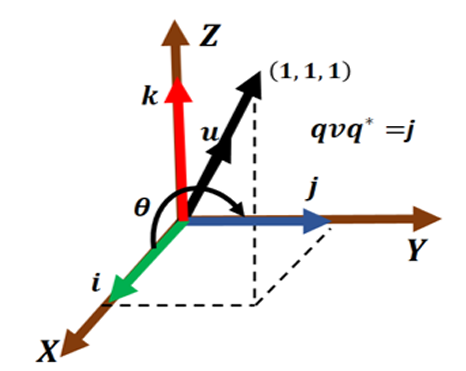
\includegraphics[width=10cm]{figure/asse2.png}
         \caption{Il quaternione q ruota il vettore v tramite un angolo ${\theta}$}
         \label{fig:asse2}
        \end{center}
    \end{figure}

    Per questo motivo, nel contesto dell'animazione e della grafica 3D si preferisce utilizzare i \textbf{quaternioni}, poichè consentono di rappresentare una rotazione tramite quattro soli numeri reali: tre per definire un asse e uno per l'angolo di rotazione.

    Un vettore ${v}$ ${\in}$ ${ \mathbb{R}^3 }$ può essere interpretato come un \textbf{quaternione puro}, ossia un quaternione con parte reale nulla. Considerando un quaternione unitario nella forma:
    \begin{align*}
        q = q_0 + {q_1}i + {q_2}j + {q_3}k = q_0 + q,
    \end{align*}

    con norma pari a 1, esiste un unico angolo ${\theta}$ \in [0, ${\pi}$] tale che:
    \begin{align*}
        q_0 = \cos{(\theta/2)} , |q| = \sin{(\theta/2)}
    \end{align*}

    Il quaternioni può quindi essere riscritto come: 
    \begin{align*}
        q = {\cos{(\theta/2)} + u\sin{(\theta/2)}}
    \end{align*}

    dove u è un vettore unitario che rappresenta l'asse di rotazione

    Definiamo ora un operatore che applica una rotazione a un vettore v mediante il prodotto quaternionico: 
    \begin{align*}
        L_q(v) = q v q^*,
    \end{align*}

    dove ${q^*}$ è il coniugato di q.

    Tale operatore presenta due proprietà fondamentali:
    \begin{enumerate}
        \item \textbf{Preserva la lunghezza del vettore}, quindi la trasformazione è isometrica: 
        \begin{align*}
            | L_q(v) | = |v|
        \end{align*}
        \item \textbf{Lascia invariati i vettori paralleli all'asse di rotazione}: se v è proporzionale a u, allora ${L_q(v) = v}$
    \end{enumerate}

    Queste proprietà dimostrano che l'operatore ${L_q}$ applica esattamente una rotazione di ampiezza $\theta$ attorno all'asse u ~\cite{quater3}. La compatezza e stabilità di tale rappresentazione la rendono particolarmente adatta alle applicazioni interattive.

    L'introduzione dei quaternioni ha permesso di superare queste limitazioni offrendo un modello matematicamente più stabile e continuo. Le principali motivazioni alla base del loro impiego sono le seguenti:

    \begin{itemize}
        \item Assenza di gimbal lock: poiché le rotazioni non dipendono da una sequenza ordinata di assi.
        \item Interpolazione fluida tra due orientamenti (nota come Spherical Linear Interpolation, o SLERP): fondamentale per animazioni continue.
        \item Maggiore stabilità numerica, utile in simulazioni e ambienti tridimensionali complessi
        \item Efficienza computazionale: le operazioni di composizione e inversione risultano più leggeree rispetto alle trasformazioni basate su matrici 3x3 o 4x4.
        \item Compatibilità con i moderni motori grafici: la maggior parte dei software di animazione 3D e dei motori di rendering utilizza internamente i quaternioni per gestire rotazioni e interpolazioni.
    \end{itemize}

    In sintesi, i quaternioni costituiscono un'evoluzione naturale rispetto agli angoli di Eulero, fornendo una rappresentazione più robusta, coerente e adatta alla manipolazione continua degli orientamenti nello spazio tridimensionale.

\section{Rigging e Skinning}

L'animazione di un personaggio digitale si basa sull'associazione tra la sua superficie visibile (mesh) e una struttura articolata interna (scheletro). Il processo che permette questa associazione è noto come rigging e consiste nell'allineare lo scheletro alla mesh e nel definire i pesi di skinning, i quali stabiliscono come il movimento di ciascun giunto influisca sui vertici della superficie. ~\cite{asmr}
Quando si utilizzano dati di motion capture, può essere necessario adattare lo scheletro affinchè rispetti le proporzioni della mesh, per poi trasferire (retargeting) il movimento originale al nuovo scheletro.
In questo contesto, la configurazione dello scheletro riguarda sia le sue caratteristiche geometriche (come scala e lunghezza delle ossa) sia la sua struttura gerarchica (numero e disposizione dei giunti). Allo stesso modo, la configurazione della mesh comprende sia le sue proporzioni volumetriche sia la topologia dei vertici che la compongono.

\subsection{Concetto di scheletro e relazione con la mesh}

Lo scheletro consiste in un insieme di giunti, come si evidenza in figura~\ref{fig:uma} (o joint) organizzati in modo gerarchico. Ogni giunto possiede:
\begin{itemize}
    \item una posizione nella posa di riposo (rest pose)
    \item una trasformazione locale rispetto al giunto "genitore"
    \item una trasformazione globale, ottenuta moltiplicando le trasformazioni lungo la gerarchia
\end{itemize}

\begin{figure}[H]
        \begin{center}
         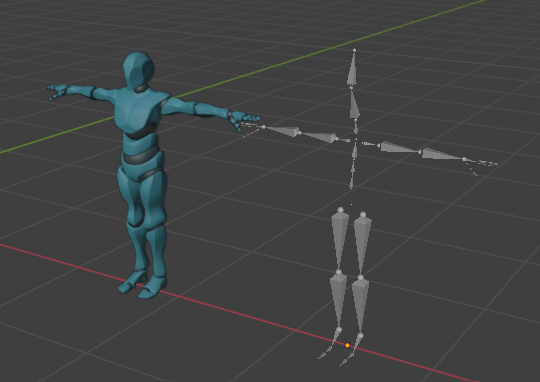
\includegraphics[width=8cm]{figure/umanoide.png}
         \caption{Mesh e scheletro umanoide}
         \label{fig:uma}
        \end{center}
    \end{figure}

La gerarchia consente di propagare il movimento: se il bacino ruota, anche la colonna, la testa e le gambe seguono coerentemente. Questo modello prende il nome di rig scheletrico.

La mesh rappresenta invece la superficie visibile del modello ed è formata da un insieme di vertici: 
\begin{align*}
    V_r \in \mathbb{R}^{{N_v}x3}
\end{align*}
dove \(N_v\) è il numero totale di vertici della mesh
Questi vertici descrivono la forma dell'oggetto nella sua posa di riposo.

Per far muovere la mesh insieme allo scheletro si utilizza un processo detto skinning, dove ogni vertice è associato a uno o più giunti tramite pesi di influenza:
\begin{align*}
    {w_{ij}} \geq 0   ,    \sum_{j=1}^{N_j} {w_{ij}} = 1
\end{align*}
dove:
\begin{itemize}
    \item \({w_{ij}}\) indica quanto il giunto j influenza il vertice i
    \item  \(N_j\) è il numero di giunti
\end{itemize}

\subsection{Linear Blend Skinning (LBS): formulazione matematica e limiti}

Il \textit{Linear Blend Skinning}(LBS) è ampiamente utilizzato nei videogiochi e in moltre applicazione real-time per deformare la superficie di un personaggio in base al movimento di un sottostante scheletro astratto.
Consideriamo un modelli deformabile rappresentato da una mesh, i cui vertici in coordinate omogenee sono indicate come $\vec{V} = \vec{v_n} \in \mathbb{R}^{4}$.

Il processo di deformazione secondo LBS puo essere definito come: 

\begin{align*}
    \tilde{v}_n = [\sum_b {w_{bn}}{B_b}]\bar{v}_n
\end{align*}

dove l'insieme delle trasformazioni omogenee \(B_b\) $\in$ $\mathbb{R}^{4x4}$ viene combinato tramite i pesi di skinning \(w_{bn}\).
Normalmente questi pesi sono dipinti manualmente da un artista digitale direttamente sulla superficie del modello; tuttavia, esistono anche algoritmi automatici per i casi in cui è richiesta una minore precisione o si desidera ridurre il tempo di produzione.

Ogni matrice di trasformazione \(B_b\) è solitamente fattorizzata nel prodotto di due trasformazioni:
\begin{align*}
    B_b = \tilde{B}_b\bar{{B}_b}^{-1}
\end{align*}
Useremo - per indicare grandezze nello \textbf{stato di riposo}(rest pose), e $\sim$ per indicare grandezze nello \textbf{stato deformato}(posed).
Le trasformazioni $\bar{B}_b^{-1}$ sono definite nella rest pose e rimangono costanti durante tutto il processo di deformazione, mentre le trasformazioni $\tilde{B}_b$ sono calcolate in funzione dei parametri di posa $\theta$, che possiamo astrarre con la funzione: 
\begin{align*}
    \{\tilde{B_b}\} = pose(\theta)
\end{align*}

Dato un vertice in rest pose $\bar{v} \in \bar{V}$, la trasformazione:
\begin{align*}
    \tilde{v}_B = \tilde{B_b}\bar{B_v}^{-1}\bar{v}
\end{align*}
esegue due operazioni:
\begin{enumerate}
    \item \textbf{Codifica locale}: $\bar{v_b}=\bar{B_b}^{-1}\bar{v}$, che esprime il punto nel sistema di riferimento locale dell'osso b.
    \item \textbf{Decodifica globale}: $\tilde{v_b}=\tilde{B_b}\bar{v_b}$, che esprime il punto nel sistema di riferimento globale nella posa corrente.
\end{enumerate}

Infine, rappresentando i pesi $w_n = \{w_n\}^*$ e le trasformazioni \(B(\theta) = \{B_b\}\) in forma tensoriale, possiamo sintetizzare lo skinning di un singolo vertice come:

\begin{align*}
    \tilde{v}_n = [w_nB(\theta)]\bar{v}_n
\end{align*}

dove \(B(\theta)\) ha dimensioni B x 4 x 4, e \(w_n\) ha dimensioni 1 x B.
Notiamo anche che i pesi \(w_n\) sono normalmente normalizzati affinchè siano \textbf{positivi} e \textbf{sommino a uno}, condizioni necessaria per ottenere una deformazione stabile e priva di artefatti.~\cite{lbs}

\paragraph{Limite dell'LBS}
Nonostante la sua semplicità ed efficienza, l'LBS presenta alcune limitazioni note:
\begin{enumerate}
    \item Collasso del volume (Candy Wrapper Problem)
    
    In presenza di rotazioni ampie, ad esempio la rotazione del braccio o di una gamba, la mesh tende a schiacciarsi invece di mantenere il volume reale.
    \item Deformazioni innaturali nelle articolazioni
    
    Le regioni vicino alle giunture (es. gomito, ginocchio) possono assumere forme troppo morbide o eccessivamente elastiche.
    \item Difficoltà nella preservazione dei dettagli
    
    LBS non tiene conto della struttura anatomica o materiale: pelle, muscoli o superfici rigide vengono trattati allo stesso modo.
\end{enumerate}

\subsection{Weight Painting e associazione ossa-vertici}

Una volta definito lo scheletro, la mesh deve essere collegata ai giunti in modo che ogni movimento delle ossa si rifletta sul modello. Questo collegamento è realizzato tramite l'assegnazione di pesi ai vertici (skinning weights). 
Ogni vertice della mesh appartiene a uno o più vertex group, ciascuno associato a un osso.
Il peso \({w_{ij}}\) indica quanto l'osso j influenza il vertice i.
\begin{align*}
    0 \leq {w_{ij}} \leq 1     ,   \sum_{j} {w_{ij}} = 1
\end{align*}
Un peso elevato implica una maggiore deformazione del vertice quando l'osso si muove. La distribuzione dei pesi può essere:
\begin{figure}[H]
        \begin{center}
         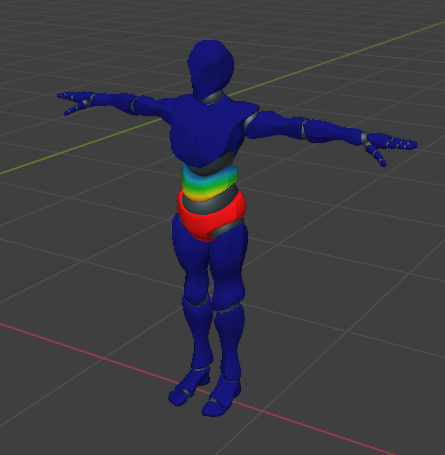
\includegraphics[width=6cm]{figure/weight.png}
         \caption{Assegnazione dei pesi}
         \label{fig:we}
        \end{center}
    \end{figure}
\begin{itemize}
    \item \textbf{Automatica}, tramite algoritmi di skinning (es. Automatic Weights in Blender),
    \item \textbf{Manuale}, tramite Weight Painting, dove il modellatore "dipinge" sulla mesh le zone di influenza delle varie ossa.
\end{itemize}

La corretta assegnazione dei pesi (figura~\ref{fig:we}) è essenziale per ottenere una deformazione naturale nelle zone articolate, come gomiti e ginocchia. Una pesatura scorretta provoca artefatti come collasso del volume, stiramenti e separazioni visibili tra le superficie. Blender visualizza i pesi con una codifica cromatica: 


\begin{table}[h]
\centering
    \begin{tabular}{|c|c|}
    \hline
    \textbf{Colore} & \textbf{Significato} \\ \hline
    Blu   & Nessuna influenza (peso $\approx 0$) \\ \hline
    Verde & Influenza moderata (peso $\approx 0.5$) \\ \hline
    Rosso & Massima influenza (peso $\approx 1$) \\ \hline
    \end{tabular}
    \caption{Scala cromatica dei pesi nel Weight Painting.}
\end{table}

Negli ultimi anni, la ricerca ha introdotto metodi che mirano ad automatizzare ulteriormente questo processo, riducendo la necessità di intervento manuale e migliorando la qualità dello skinning anche su mesh complesse. Tra questi, si distinguono approcci basati su modelli generativi e apprendimento automatico. Ad esempio, alcuni sistemi recenti, come \textbf{UniRig} ~\cite{uni}, propongono un generatore unico in grado di produrre scheletri e pesi di skinning coerenti partendo dalla sola geometria della mesh. In modo simile, metodi come \textbf{ASMR} ~\cite{asmr} introduco strategie adattive per prevedere automaticamente la distribuzione dei pesi, sfruttando descrittori geometrici avanzati per individuare le aree di articolazione.

Sebbene tali tecniche non sostituiscano completamente le procedure tradizionali, rappresentano un'evoluzione importante nelle pipeline di rigging moderne, offrendo soluzioni più robuste e generalizzabili e riducendo i tempi di preparazione dei modelli. In questo senso, lo skinning non è più solo un processo manuale, ma si colloca all'interno di un più ampio panorama di metodi automatizzati che mirano a rendere la deformazione della mesh più accurata, stabile e riutilizzabile.


\section{Retargeting dell'animazione}

Il retargeting dell'animazione è il processo con cui un'animazione definita su un personaggio (sorgente) viene trasferita su un altro (target), anche quando i due modelli presentano differenze nella forma, nelle proporzioni o nella struttura dello scheletro.
Questo procede richiede: 

\begin{enumerate}
    \item Allineamento degli scheletri (mappatura articolazioni S $\rightarrow$ T)
    \item Adattamento delle proporzioni (bone scaling)
    \item Trasferimento del movimento nel tempo (rotazioni + posizioni articolari)
\end{enumerate}

Storicamente, il retargeting veniva eseguito manualmente tramite Inverse Kinematics e regolazioni osso per osso.
Oggi, esistono metodi automatici che combinano:
\begin{itemize}
    \item analisis strutturate dello scheletro,
    \item ottimizzazione sui pesi dello scheletro,
    \item apprendimento automatico.
\end{itemize}

Tra gli approcci moderni spiccano UniRig e ASMR, che permettono di trasferire animazioni anche su modelli non umanoidi, generalizzando la pipeline oltre il classino personaggio bipede.

\subsection{Concetto di motion retargeting tra modelli diversi}
Il motion retargeting è il processo attraverso il quale un'animazione originariamente associata a un determinato modello o scheletro viene trasferita a un personaggio con proporzioni o struttura differente. La difficoltà principale consiste nel preservare la coerenza del movimento, evitando deformazioni innaturali e garantendo la stabilità del risultato.
Con l'evoluzione del machine learning, sono stati studiati approcci che sfruttano reti neurali per apprendere direttamente la mappatura tra scheletri differenti, riducendo la necessità di progettare manualmente vincoli cinematici o modelli di ottimizzazione. Alcuni di questi metodi integrano Forward Kinematics in architetture ricorrenti e introducono vincoli di ciclo per preservare la coerenza del movimento durante la trasformazione.
In sintesi, il motion retargeting si è evoluto da metodi basati su ottimizzazione e IK a soluzioni neurali che apprendono direttamente lo spazio delle pose, con l'obiettivo di gestire scheletri eterogenei e movimenti complessi in modo più robusto ed automatizzato.

\subsection{Introduzione ai metodi automatici: UniRig e ASMR come approcci moderni}
Negli ultimi anni, il campo del motion retargeting ha visto la diffusione di metodi automatici capaci di trasferire animazioni tra personaggi con proporzioni corporee o strutture scheletriche differenti, riducendo al minimo l'interveto manuale. Questi approcci sfruttano modeli statistici o reti neurali per apprendere la relazione tra pose, scheletri e deformazioni della mesh, con l'obiettivo di preservare la naturalezza del movimento durante il trasferimento.
Tra i metodi recenti, si possono distinguere due linee principali:

\paragraph{Metodi basati su adattamento geometrico (es. UniRig)}

approccio come \textbf{UniRig} mirano a costruire automaticamente uno scheletro coerente con la forma della mesh. L'idea è quella di estrarre informazioni geometriche dal modello (es. esempio simmetria, volumi e articolazioni visive) per posizionare le articolazioni in modo plausibile. Successivamente, vengono calcolati i pesi di skining e l'animazione può essere trasferita da altri oggetti.
Questi metodi sono particolarmente utili quando si lavora con mesh prive di rig o quando si devono riggare personaggi eterogenei in modo uniforme.

\paragraph{Metodi basati su apprendimento (es. ASMR)}

approcci come ASMR utilizzano reti neurali per apprendere direttamente il processo di retargeting. Il modello  è addestrato su numerosi esempi di movimenti eseguiti da scheletri differenti, imparando a mantenere la coerenza del gesto indipendentemente dalla struttura del personaggio.
Rispetto ai metodi puramente geometrici, tali tecniche possono adattare automaticamente lo stile del movimento e ridurre distorsioni o artefatti durante la deformazione.

In sintesi UniRig e ASMR rappresentano due direzioni complementari nel motion retargeting moderno:
\begin{itemize}
    \item l'una focalizzata sulla costruzione automatica dello scheletro e del sistema di skinning,
    \item l'altra sull'apprendimento della trasformazione del movimento
\end{itemize}
Entrambi contribuiscono a rendere l'animazione più accessibile, riducendo tempo e complessità nelle pipeline di produzione.




